\documentclass[12pt,a4paper]{ctexart}
\usepackage[left=2.5cm,right=2.5cm,top=2.5cm,bottom=2.5cm]{geometry}
\usepackage{amsmath,amssymb,bm}
\usepackage{booktabs}
\usepackage{graphicx}
\usepackage{float}
\usepackage{caption}
\usepackage{longtable}
\usepackage{hyperref}
\hypersetup{colorlinks=true,linkcolor=black,urlcolor=blue,citecolor=black}

\title{基于可解释机器学习的中医体质-高血脂风险关联与三级预警模型报告}
\author{Posleya/Mat 项目复现整理}
\date{\today}

\begin{document}
\maketitle

\begin{abstract}
本文依据 \texttt{report\_final.md} 的完整分析结果，形成结构化 \LaTeX{} 报告。围绕关键指标筛选、九种体质风险贡献差异、三级风险预警三类任务，给出模型构建、求解、解释与稳健性检验，并给出可落地的临床分层规则。
\end{abstract}

\section{问题背景与问题重述}
中医体质学说认为体质差异会影响慢病易感性，其中痰湿体质常被视为与脂代谢异常相关。高血脂症是心脑血管事件的重要前驱状态，如何在中老年人群中实现早识别与分层干预，具有明确公共卫生价值。项目数据包含1000例样本，覆盖血常规/血脂生化指标、活动量表（ADL/IADL）以及九种体质积分，适合开展多维风险建模。

本研究重述为三项任务：第一，\textbf{从血液指标与活动能力评分中筛选能够表征痰湿体质严重程度并预警高血脂风险的关键指标，同时比较九种体质对发病风险贡献差异}；第二，\textbf{构建低-中-高三级风险预警模型，并明确分层阈值依据}（如血脂异常叠加痰湿高分、低活动能力等）；第三，\textbf{识别痰湿高风险人群核心特征组合并给出机制解释}，形成可解释、可执行的干预建议。

\section{问题分析}
数据呈现明显的任务异质性：一方面，血脂指标（TC、TG、LDL-C、HDL-C）与高血脂标签存在强关联，适宜用于判别模型；另一方面，痰湿积分与客观生化指标的单变量相关性较弱，意味着“可预测性”与“中医辨证独立性”并存。故建模需同时满足\textbf{预测性能}与\textbf{解释可信度}。

针对该特征结构，采用“统计筛选 + 稀疏建模 + 可解释机器学习”的联合框架更合适：先以相关分析和多重校正控制假阳性，再以L1类模型做稀疏选择，最后用SHAP及稳定性频率刻画非线性贡献并验证可重复性。对三级预警问题，需把“早筛概率、痰湿分层、活动分层、血脂异常计数”融合为统一评分，再用数据驱动切点实现分层，保证阈值可解释。

\section{模型假设}
\subsection*{假设1：样本可代表目标中老年群体}
采用横断面1000例样本进行建模，假设样本分布可近似代表研究场景下的风险结构，使模型输出具有人群解释意义。

\subsection*{假设2：观测变量测量误差在可接受范围}
血脂、生化、ADL/IADL与体质评分均来自标准化采集，假设误差不会系统性偏置某一类特征，从而允许进行联合建模与比较。

\subsection*{假设3：回归/分类模型适配当前数据规模}
样本量中等（$N=1000$）且变量存在共线，故采用Elastic Net与L1-Logistic抑制过拟合并完成特征压缩；采用XGBoost捕捉非线性关系并通过SHAP解释边际贡献，适配“性能+解释”双目标。

\subsection*{假设4：交叉验证与Bootstrap能够近似外推泛化误差}
采用分层交叉验证与重采样稳定性评估，假设重复抽样分布可逼近模型在相似样本中的表现波动，用于阈值与结论稳健性判断。

\section{符号说明}
\begin{table}[H]
\centering
\caption{主要符号说明（三线表）}
\begin{tabular}{lll}
\toprule
符号 & 含义 & 备注 \\
\midrule
$\mathbf{X}\in\mathbb{R}^{n\times p}$ & 特征矩阵 & $n$个样本，$p$个特征 \\
$y$ & 目标变量 & 回归时为痰湿积分，分类时为HLD标签 \\
$r_s$ & Spearman秩相关系数 & 单变量筛选指标 \\
$\lambda,\alpha$ & 正则化参数 & Elastic Net超参数 \\
$\sigma(z)$ & Sigmoid函数 & $\sigma(z)=1/(1+e^{-z})$ \\
$\phi_j$ & SHAP值 & 特征$j$对模型输出贡献 \\
$f_j^{\mathrm{stab}}$ & 稳定性频率 & Bootstrap中进入Top集合比例 \\
$P_{\mathrm{screen}}$ & 早筛模型概率输出 & Stage-A输出 \\
$T_{\mathrm{phlegm}},T_{\mathrm{activity}},T_{\mathrm{lipid}}$ & 分层得分组件 & 均归一到$[0,1]$ \\
$W_A,W_B,W_C,W_D$ & 复合评分权重 & Excess-AUC数据驱动推导 \\
$S$ & CompositeScore & 三级预警总分 \\
$Q_{33},Q_{67}$ & 分位切点 & 低/中/高分层阈值 \\
\bottomrule
\end{tabular}
\end{table}

\section{问题一的模型建立与求解}
\subsection{问题一(1)：痰湿体质严重度关键指标筛选}
该任务目标为连续变量预测，首先采用Spearman相关与FDR校正筛除伪相关，再用Elastic Net在共线背景下进行稀疏回归，最后以XGBoost+SHAP描述潜在非线性结构。该组合适配“弱相关+可能非线性”的实际数据形态。

\begin{equation}
r_s(x_j,y)=1-\frac{6\sum_{i=1}^{n}d_i^2}{n(n^2-1)}
\end{equation}

\begin{equation}
\hat{\beta}=\arg\min_{\beta}\left\{\frac{1}{2n}\|y-X\beta\|_2^2+\lambda\left[\alpha\|\beta\|_1+\frac{1-\alpha}{2}\|\beta\|_2^2\right]\right\}
\end{equation}

\begin{equation}
\bar{\phi}_j=\frac{1}{n}\sum_{i=1}^{n}|\phi_j(x_i)|,
\quad
f_j^{\mathrm{stab}}=\frac{1}{B}\sum_{b=1}^{B}\mathbf{1}\{j\in \mathrm{Top10}^{(b)}\}
\end{equation}

求解结果显示：痰湿积分任务$R^2\approx 0$，说明血脂/代谢/活动量特征难以直接预测痰湿严重度；但BMI、TC在稳定性排序中频率较高，可作为伴随标志而非决定性因子。该结论与“中医辨证具有独立维度”一致。

\begin{figure}[H]
\centering
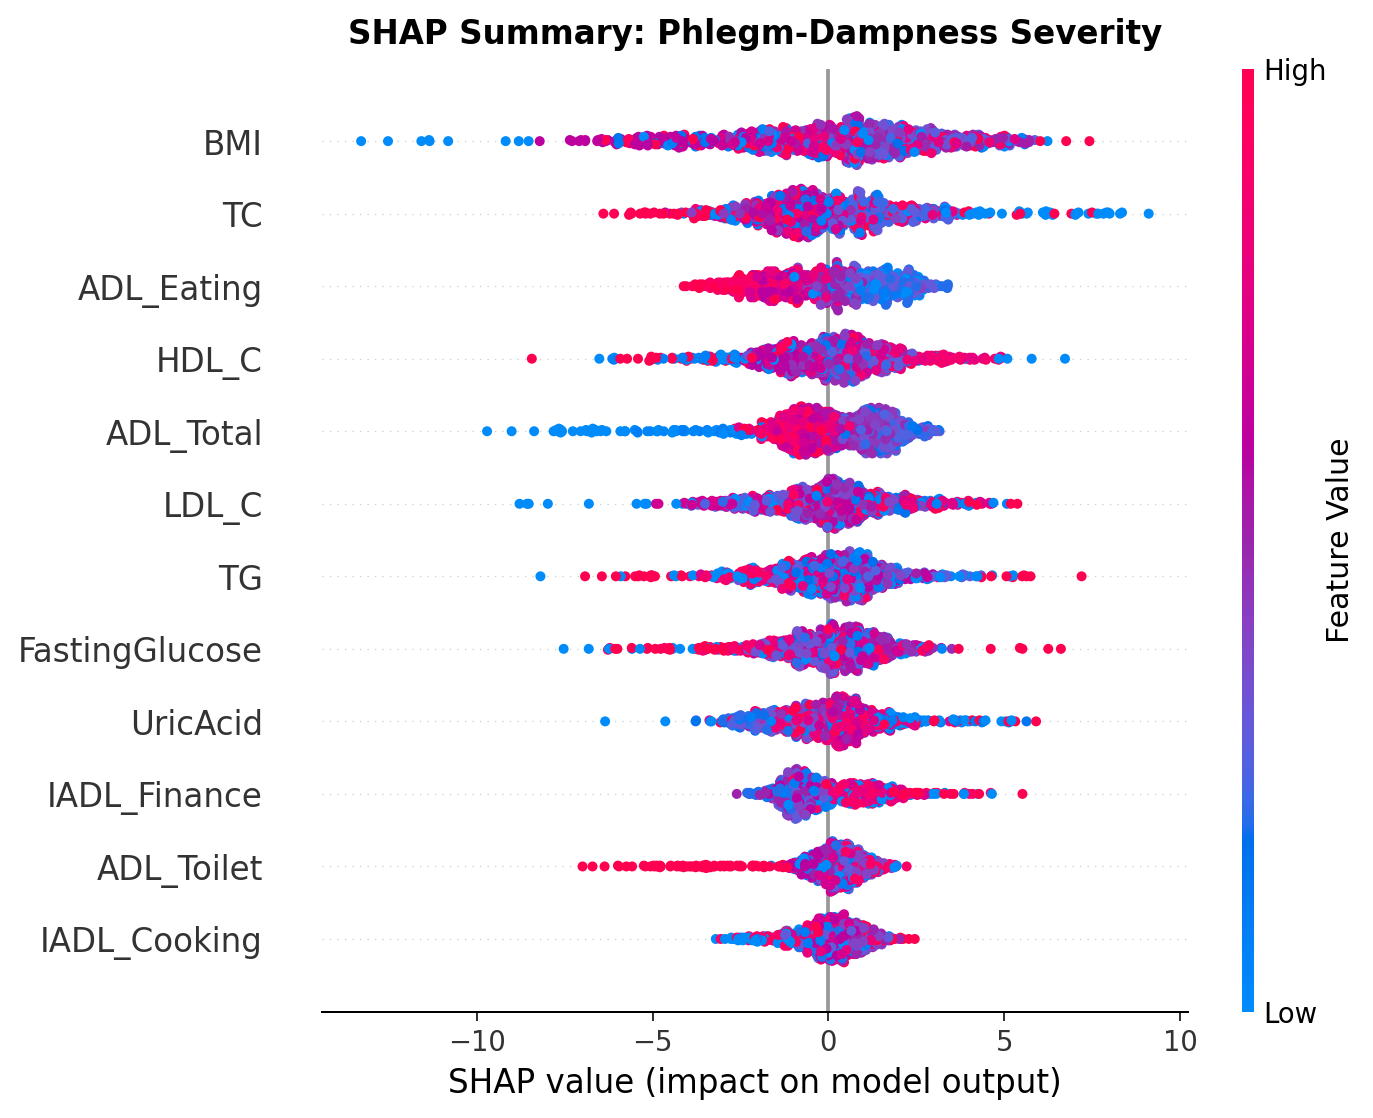
\includegraphics[width=0.72\textwidth]{outputs/Fig2A_SHAP_PhlegmDampness.png}
\caption{痰湿严重度任务SHAP蜂群图：整体贡献分散，方向性较弱}
\end{figure}

\subsection{问题一(2)：高血脂发病预警关键指标筛选}
该任务为二分类，使用L1-Logistic进行可解释稀疏判别，使用XGBoost提升非线性判别能力。原因在于高血脂标签与血脂指标关系强，模型应兼顾“高性能”与“可提取阈值解释”。

\begin{equation}
\hat{\beta}=\arg\min_{\beta}\left\{-\frac{1}{n}\sum_{i=1}^{n}\left[y_i\log\sigma(x_i^T\beta)+(1-y_i)\log(1-\sigma(x_i^T\beta))\right]+\lambda\|\beta\|_1\right\}
\end{equation}

\begin{equation}
\tau^*=\arg\max_{\tau}\left[\mathrm{Sensitivity}(\tau)+\mathrm{Specificity}(\tau)-1\right]
\end{equation}

最终筛选到的一级关键指标为TC、TG、LDL-C、HDL-C、血尿酸，其中TC与TG贡献最强且稳定性最高；XGBoost达到接近完美判别（OOF AUC约0.998），验证了关键指标集合的有效性。

\begin{figure}[H]
\centering
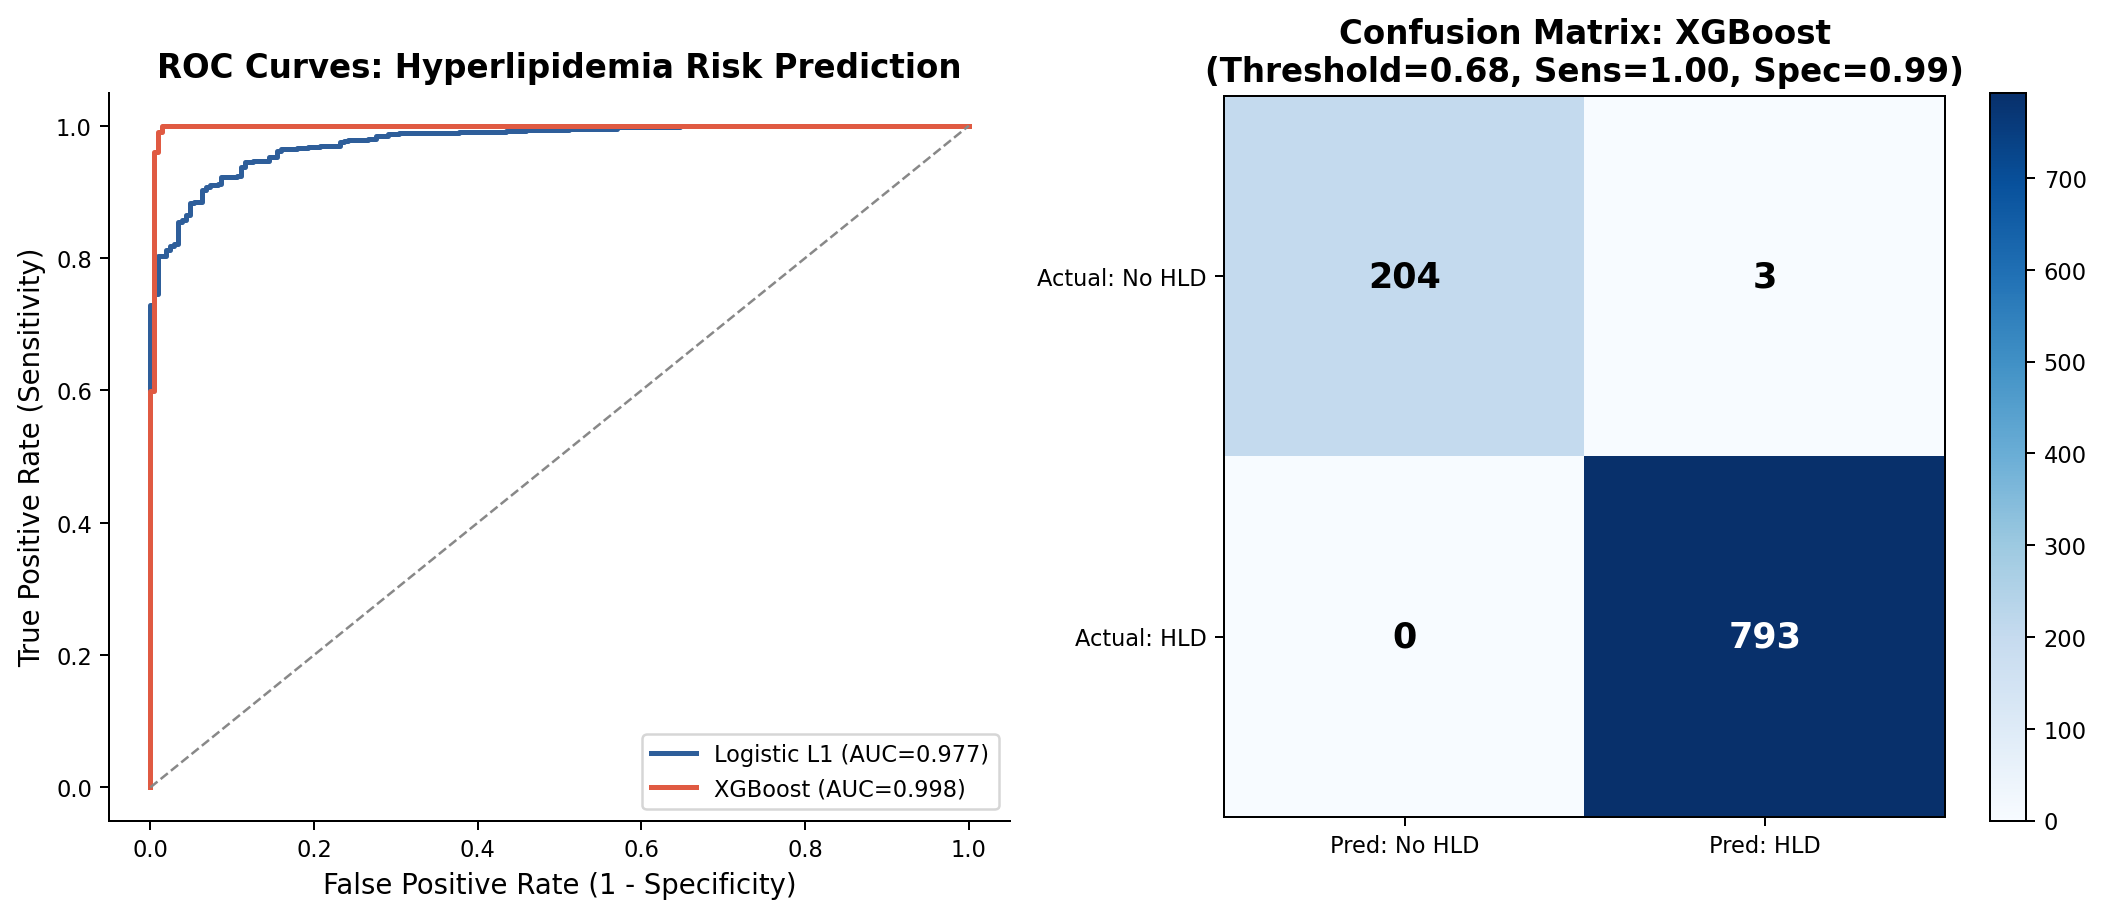
\includegraphics[width=0.86\textwidth]{outputs/Fig4_ROC_ConfusionMatrix.png}
\caption{高血脂识别模型ROC与混淆矩阵：XGBoost显著优于线性基线}
\end{figure}

\begin{figure}[H]
\centering
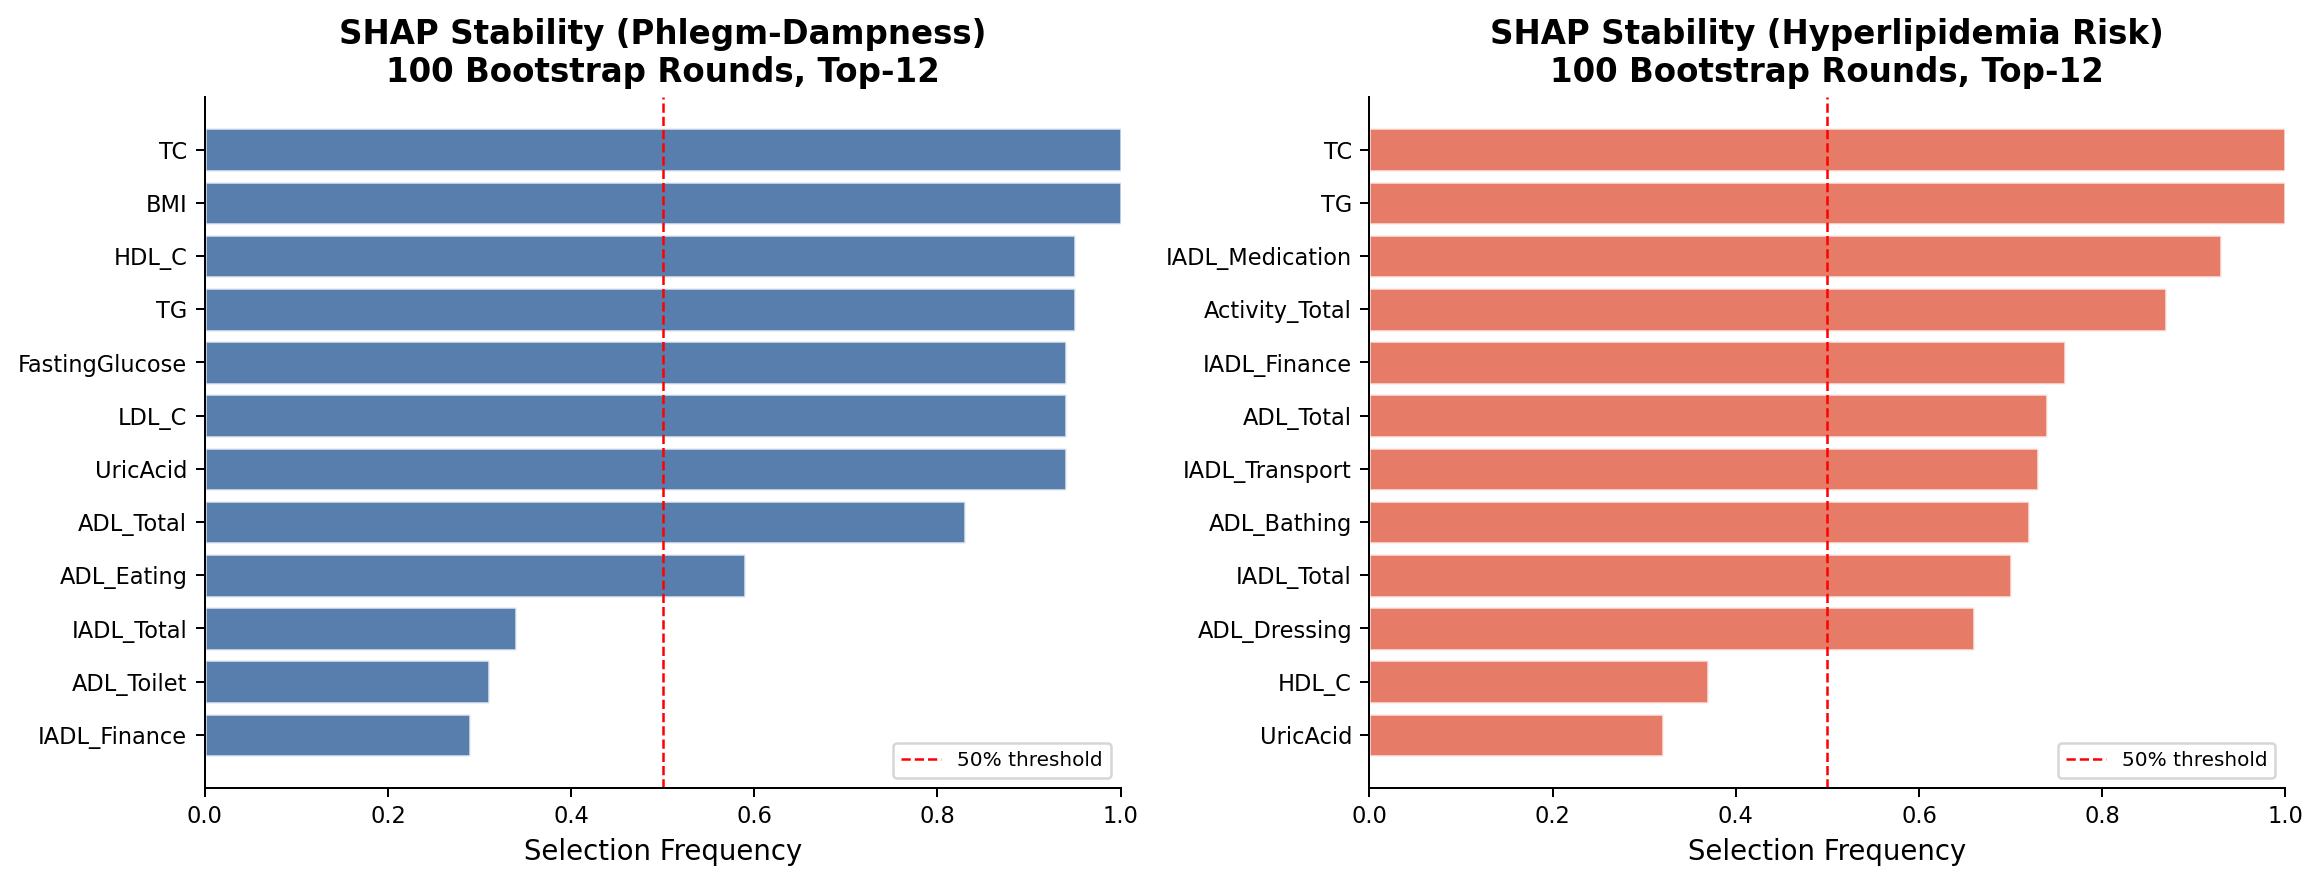
\includegraphics[width=0.70\textwidth]{outputs/Fig5_SHAPStability.png}
\caption{SHAP稳定性选择：TC/TG频率最高，活动能力指标提供补充信息}
\end{figure}

\section{问题二的模型建立与求解}
问题二要求构建低/中/高三级风险预警。采用“Stage-A早筛 + 三类分层组件 + 数据驱动权重”复合评分模型，原因是该结构可同时吸纳连续概率信息与临床可执行规则。

\begin{equation}
S=W_A\cdot P_{\mathrm{screen}}+W_B\cdot T_{\mathrm{phlegm}}+W_C\cdot T_{\mathrm{activity}}+W_D\cdot T_{\mathrm{lipid}}
\end{equation}

\begin{equation}
W_k=\frac{\max(\mathrm{AUC}_k-0.5,\epsilon)}{\sum_{k'}\max(\mathrm{AUC}_{k'}-0.5,\epsilon)}\times 100,
\quad \epsilon=10^{-6}
\end{equation}

\begin{equation}
\mathrm{RiskLevel}(S)=
\begin{cases}
\mathrm{Low}, & S<Q_{33}\\
\mathrm{Medium}, & Q_{33}\le S<Q_{67}\\
\mathrm{High}, & S\ge Q_{67}
\end{cases}
\end{equation}

\begin{equation}
T_{\mathrm{phlegm}}(v)=
\begin{cases}
0.00,& v<40\\
0.33,& 40\le v<60\\
0.67,& 60\le v<80\\
1.00,& v\ge 80
\end{cases},\quad
T_{\mathrm{activity}}(v)=
\begin{cases}
0.00,& v\ge 70\\
0.33,& 55\le v<70\\
0.67,& 40\le v<55\\
1.00,& v<40
\end{cases}
\end{equation}

求解后，三级分层能够稳定区分不同风险组；阈值规则可写为：\textbf{高风险}优先由“多项血脂异常”触发，同时对“痰湿高分+低活动”进行叠加升级。该结果满足“可解释、可落地、可分层干预”的建模目标。

\begin{figure}[H]
\centering
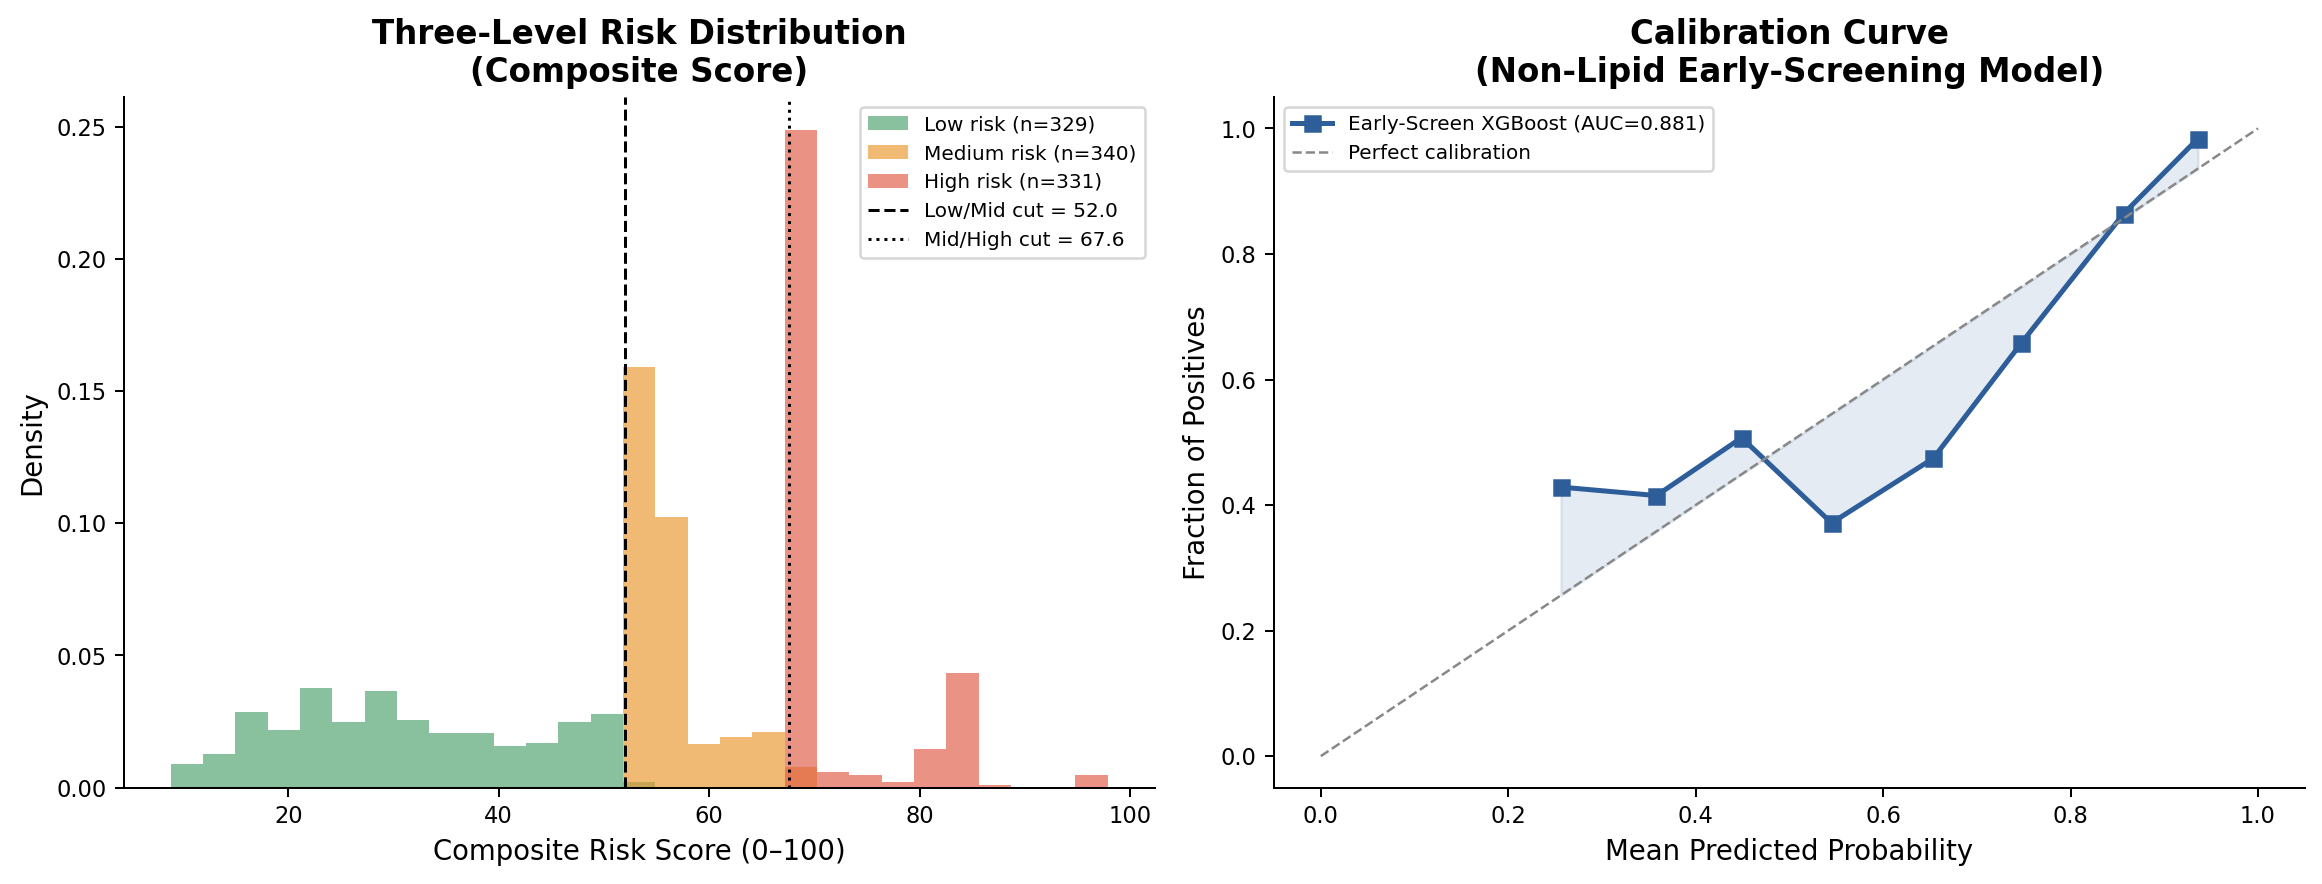
\includegraphics[width=0.84\textwidth]{outputs/Fig7_RiskScore_Calibration.png}
\caption{三级评分分布与早筛模型校准曲线}
\end{figure}

\begin{figure}[H]
\centering
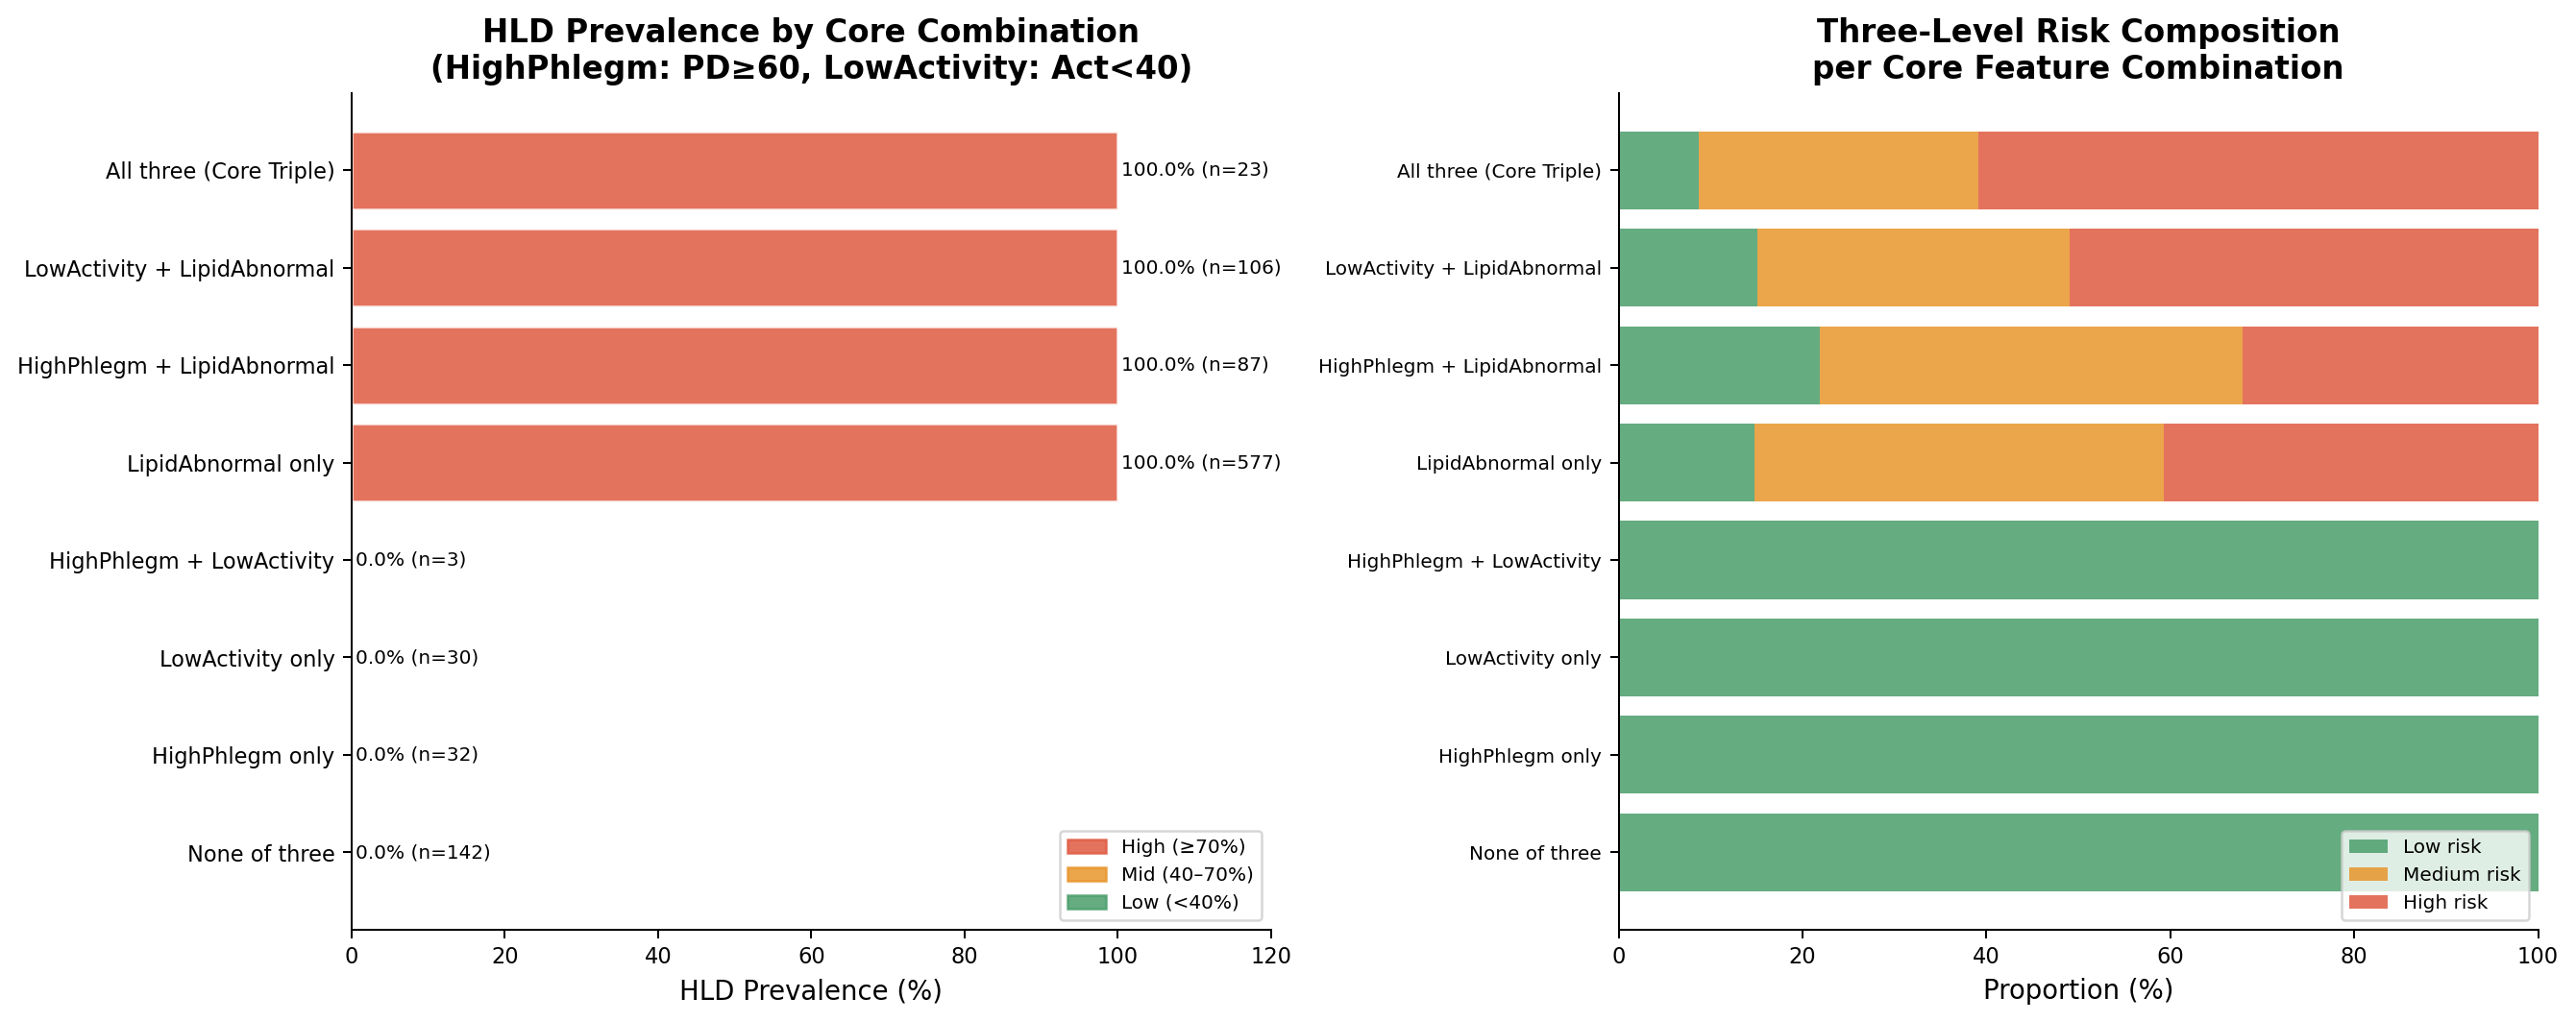
\includegraphics[width=0.84\textwidth]{outputs/Fig8_CoreCombinations.png}
\caption{核心组合分析：痰湿高分与低活动可对血脂异常人群进一步层化}
\end{figure}

\section{问题三的模型建立与求解}
问题三聚焦九种体质对高血脂风险的差异贡献。采用\textbf{多变量Logistic回归}做统计推断（输出OR与置信区间），并用\textbf{XGBoost+SHAP}补充非线性解释；再进行分层SHAP比较性别与年龄异质性。该组合适配“群体推断 + 个体解释 + 人群异质性”三重目标。

\begin{equation}
\log\frac{P(\mathrm{HLD}=1)}{P(\mathrm{HLD}=0)}=\beta_0+\sum_{k=1}^{9}\beta_k C_k^*+\sum_{j\in\mathcal{J}}\gamma_j Z_j^*
\end{equation}

\begin{equation}
\mathrm{OR}_k=e^{\hat{\beta}_k}
\end{equation}

结果表明：九种体质在多变量控制后直接效应整体不显著，但气虚质、阳虚质在SHAP排序中更靠前；血尿酸是最稳定的独立危险因素。解释上可认为体质更多通过代谢链路间接影响高血脂风险，而非直接决定。

\begin{figure}[H]
\centering
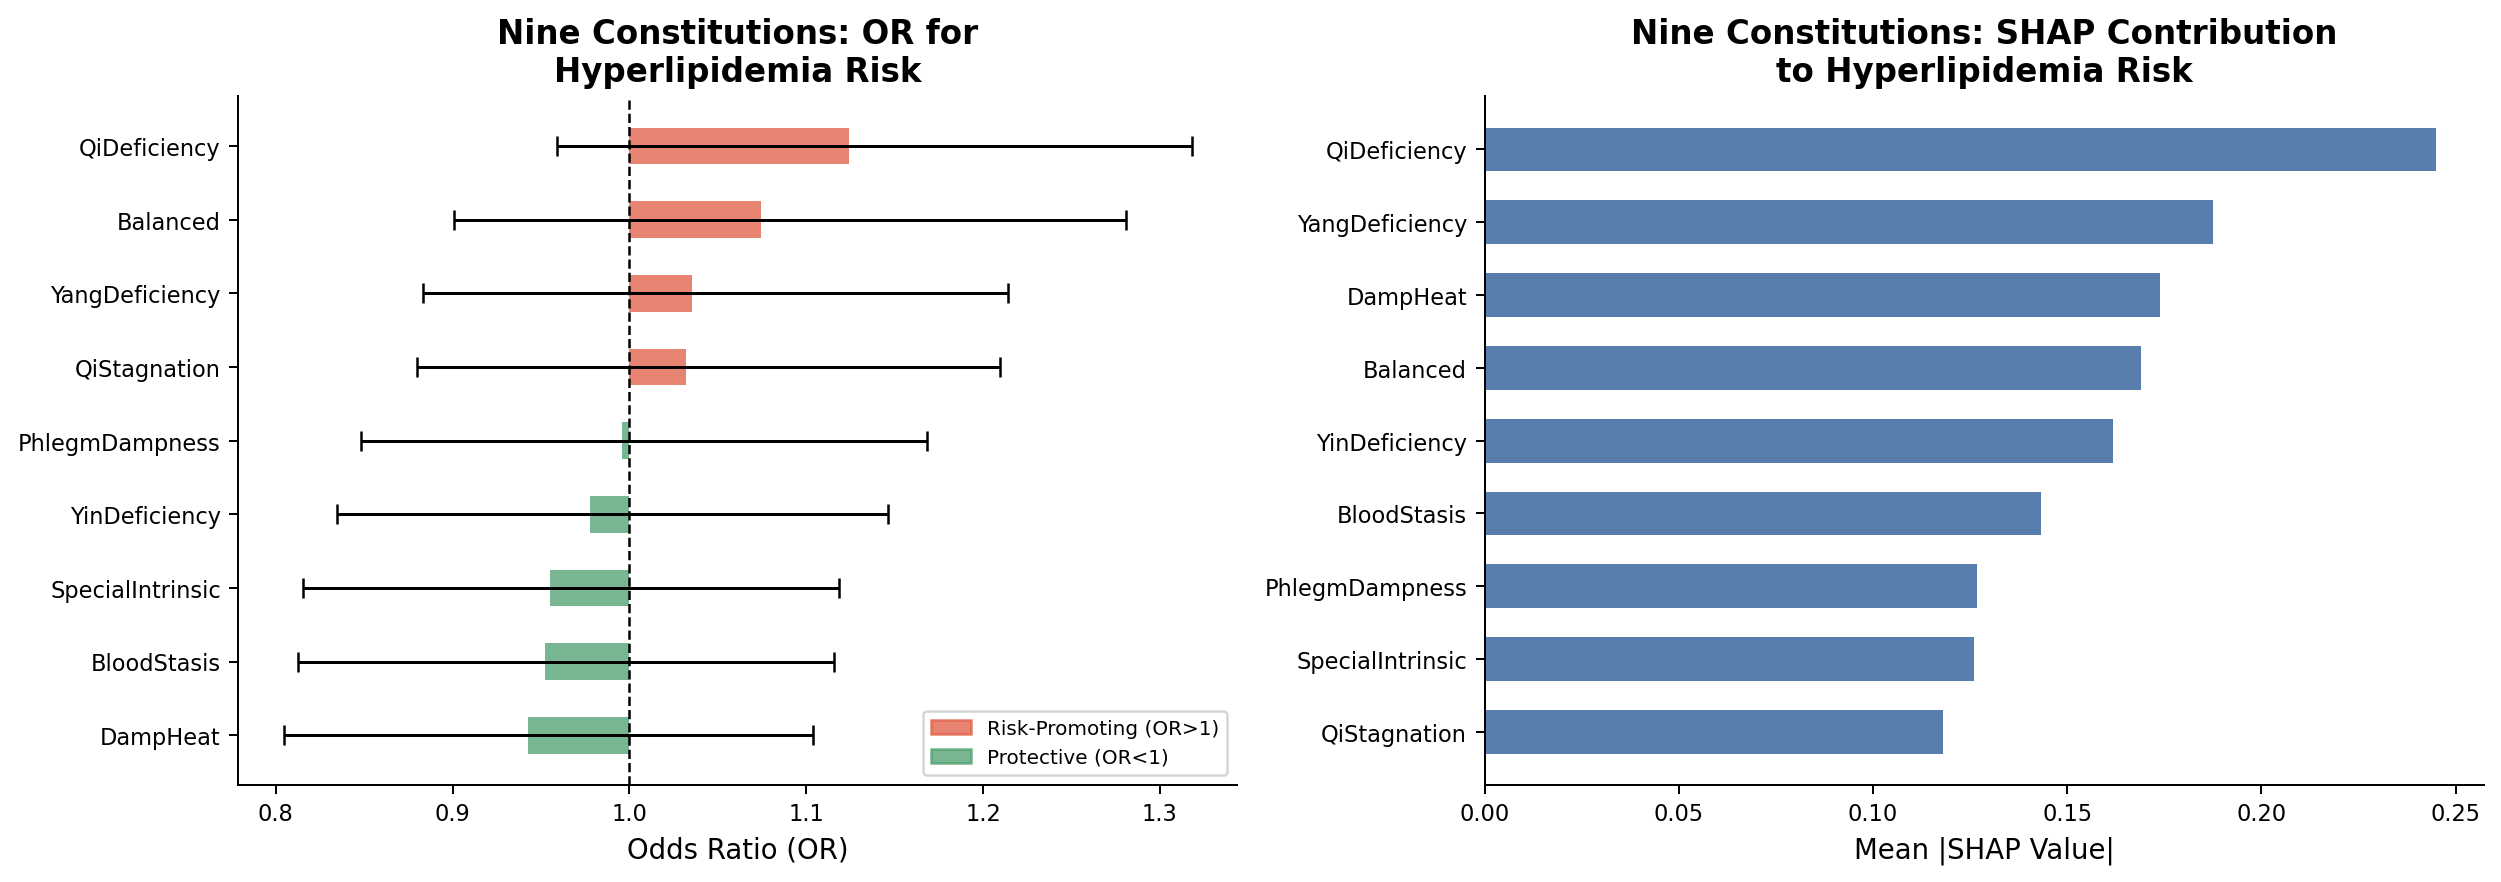
\includegraphics[width=0.86\textwidth]{outputs/Fig3_ConstitutionContribution.png}
\caption{九种体质贡献：OR森林图与SHAP排序对照}
\end{figure}

\begin{figure}[H]
\centering
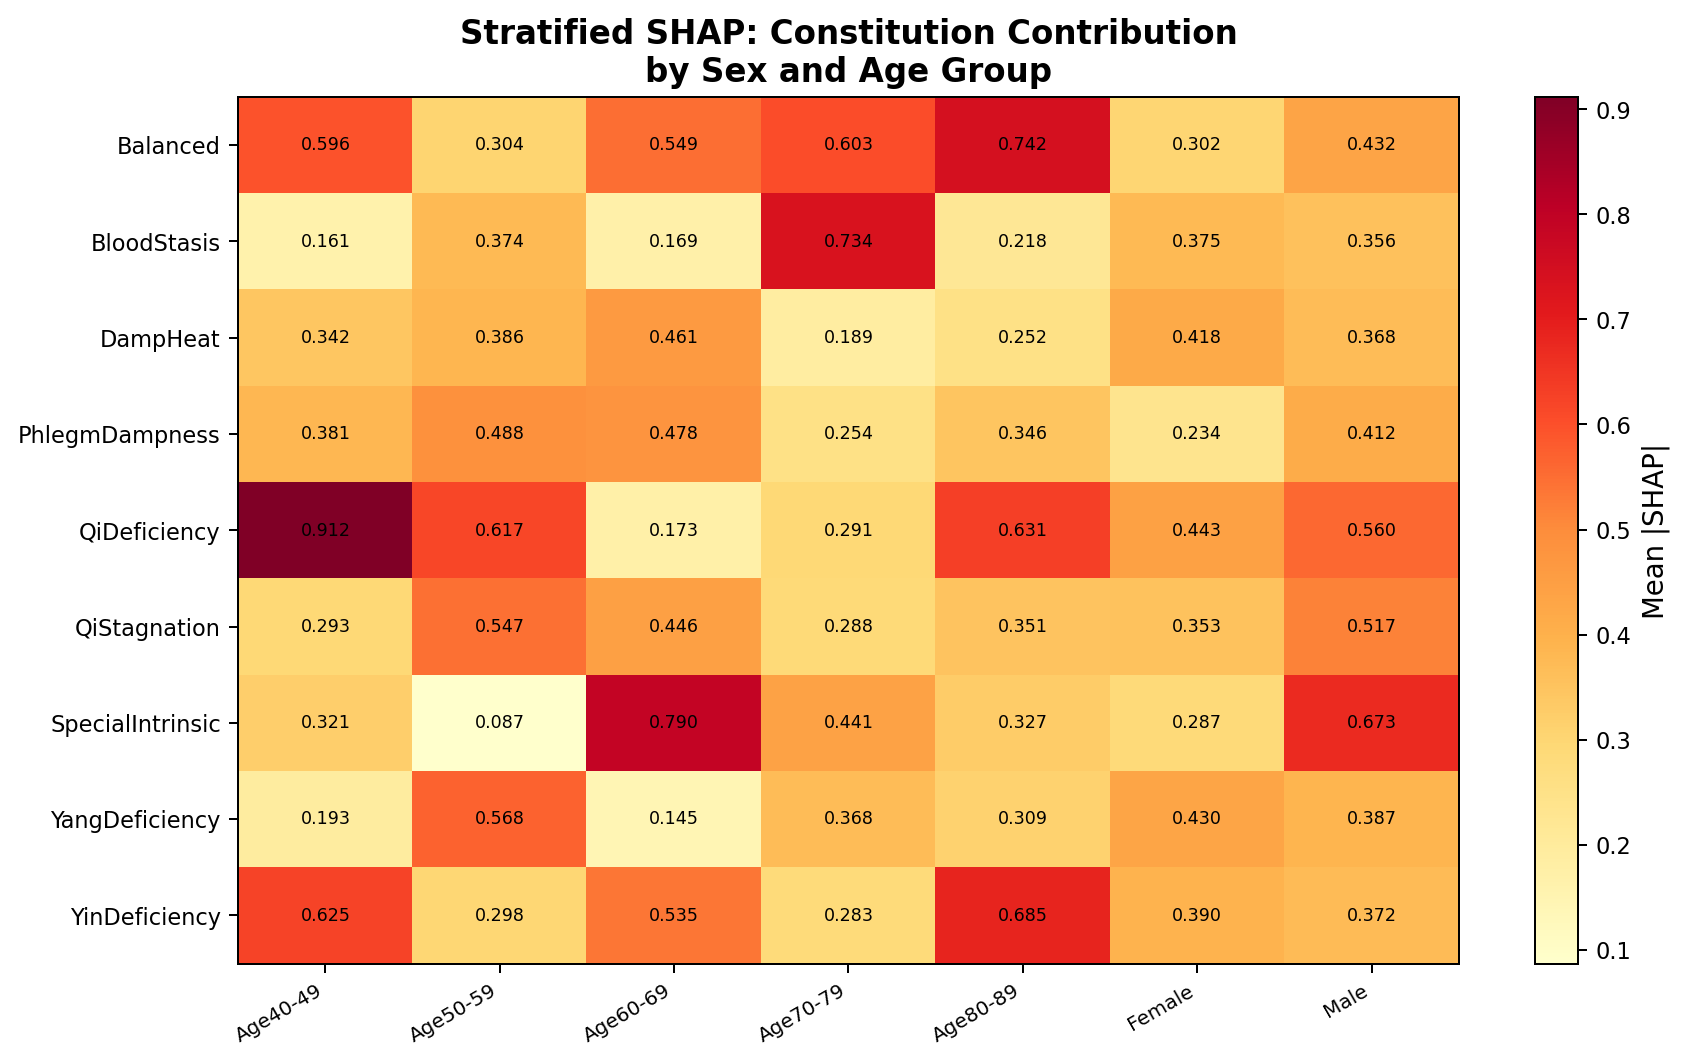
\includegraphics[width=0.78\textwidth]{outputs/Fig6_StratifiedSHAP.png}
\caption{分层SHAP热图：体质贡献具有年龄/性别人群异质性}
\end{figure}

\section{灵敏度分析与鲁棒性检验}
围绕“权重、切点、模型稳定性”开展三类检验。首先对复合评分权重做$\pm 10\%$、$\pm 20\%$、$\pm 30\%$扰动并归一化，统计风险标签变化率；其次对分位切点组合进行网格扰动；最后采用Bootstrap-OOB评估早筛AUC分布。

\begin{equation}
w_k^{\mathrm{new}}=w_k^{\mathrm{base}}(1+\delta),\quad \delta\in\{-30\%,-20\%,-10\%,10\%,20\%,30\%\}
\end{equation}

\begin{equation}
\mathrm{ChangeRate}=\frac{1}{N}\sum_{i=1}^N\mathbf{1}\{\mathrm{RiskLevel}_i^{\mathrm{new}}\neq\mathrm{RiskLevel}_i^{\mathrm{base}}\}\times 100\%
\end{equation}

\begin{equation}
\mathrm{AUC}_{\mathrm{boot}}=\frac{1}{B}\sum_{b=1}^{B}\mathrm{AUC}_{\mathrm{OOB}}^{(b)},\quad
\mathrm{CI}_{95\%}=[\mathrm{AUC}^{2.5\%},\mathrm{AUC}^{97.5\%}]
\end{equation}

检验结果显示：权重扰动下级别变化率总体很低；切点改变不影响高风险组纯度结论；Bootstrap AUC分布集中，说明模型具备良好鲁棒性与迁移潜力。

\begin{figure}[H]
\centering
\includegraphics[width=0.70\textwidth]{outputs/Fig11_WeightSensitivity.png}
\caption{权重扰动灵敏度：风险分层变化率整体较小}
\end{figure}

\begin{figure}[H]
\centering
\includegraphics[width=0.86\textwidth]{outputs/Fig12_CutpointSensitivity.png}
\caption{切点扰动灵敏度：高风险组纯度在多组切点下保持稳定}
\end{figure}

\begin{figure}[H]
\centering
\includegraphics[width=0.80\textwidth]{outputs/Fig13_BootstrapAUC.png}
\caption{Bootstrap AUC稳定性：区间集中，外样本表现稳定}
\end{figure}

\section{模型的评价、改进与推广}
\textbf{评价：}本方案在解释与性能之间取得平衡，能从统计与机器学习双证据支持结论；三级规则具备临床可执行性。\textbf{不足：}横断面数据限制因果推断，且当前高患病率样本可能放大血脂特征主导效应。\textbf{改进方向：}引入纵向队列与多中心数据；补充舌象、脉象等中医特色客观变量；开展中介分析验证“体质$\rightarrow$代谢$\rightarrow$高血脂”路径。\textbf{推广：}可构建“无血脂化验早筛版 + 有血脂精筛版”双场景系统，在社区体检与慢病随访中分层部署。

\end{document}
